\documentclass[11pt,a4paper]{article}
\usepackage[a4paper,margin=2.6cm]{geometry}
\usepackage{iftex}
\ifPDFTeX
  \usepackage[T2A]{fontenc}
  \usepackage[utf8]{inputenc}
  \usepackage[russian]{babel}
\else
  \usepackage{fontspec}
  \usepackage{polyglossia}
  \setdefaultlanguage{russian}
  \setotherlanguage{english}
  \defaultfontfeatures{Ligatures=TeX}
  \setmainfont{Times New Roman}
  \setsansfont{Arial}
  \newfontfamily\cyrillicfont{Times New Roman}
  \newfontfamily\cyrillicfontsf{Arial}
  \setmonofont{Courier New}
  \newfontfamily\cyrillicfonttt{Courier New}
\fi
\usepackage{microtype}
\usepackage{mathtools,amssymb}
\usepackage{graphicx}
\usepackage{booktabs}
\usepackage{float}
\usepackage{caption}
\captionsetup{font=small,labelfont=bf}
\usepackage{enumitem}
\setlist{nosep,leftmargin=1.5em}
\usepackage{csquotes}
\usepackage[backend=biber,style=numeric-comp,sorting=none,maxbibnames=6]{biblatex}
\addbibresource{references_v2.bib}
\usepackage[unicode,hidelinks]{hyperref}
\setlength{\emergencystretch}{2em}

\title{Региональные инварианты межмасштабной организации атмосферной циркуляции:\\
сопряжённость иерархических уровней и асимметрия межуровневого переноса\\
по данным реанализов}
\author{Сотириади Н.}
\date{2026}

\begin{document}
\maketitle

\begin{abstract}
Работа посвящена вопросу, обладает ли регион устойчивым «почерком» взаимодействия пространственных уровней атмосферной циркуляции, не сводимым к спектру мощности. Развивая линию школы Ю.\,Г.~Пузаченко --- от выделения иерархических уровней организации геосистем к измерению их взаимодействия, --- мы строим два компактных дескриптора поля относительного вихря на уровне 850~гПа: профиль сопряжённости соседних октавных уровней $P$ (пространственная ранговая корреляция карт активности уровней) и индекс асимметрии межуровневого переноса $A$ (мера невзаимности статистических операторов агрегирования и детализации). На материале ERA5 (12 регионов размером $20^\circ\times40^\circ$ в шести циркуляционных режимах, сезоны январь--март и июль--сентябрь 2017--2024~гг.) в рамках программы заранее фиксируемых протоколов с подтверждением на независимых по годам выборках показано: оба дескриптора образуют устойчивые региональные сигнатуры ($p=0{,}001$); индекс~$A$ несёт информацию сверх спектра мощности и сверх профиля~$P$ и устойчив к контролям геометрии областей и эффективного разрешения реанализа. Региональная география индекса~$A$ воспроизводится в независимом реанализе MERRA-2 (ранговая корреляция $\rho=0{,}93$, $p<10^{-4}$), что исключает интерпретацию инварианта как артефакта конкретной системы усвоения данных. Максимальные значения $A$ приурочены к влажно-конвективным океаническим режимам, минимальные --- к аридным континентальным. Приводится полный каталог отрицательных результатов программы; центральное эмпирическое утверждение предшествующей публикации автора ретрагируется с указанием причин. Обсуждается значение асимметрии межуровневого переноса как измеримой характеристики необратимости географического обобщения и её возможная связь с региональными пределами предсказуемости атмосферы.
\end{abstract}

\section{Введение}
\label{sec:intro}

\subsection{Иерархическая организация геосистем и проблема инвариантов}

Представление о геосистемах как об иерархически организованных образованиях, в которых процессы разных пространственно-временных уровней связаны, но не сводимы друг к другу, принадлежит к числу основополагающих в отечественной теоретической географии. В работах Ю.\,Г.~Пузаченко эта идея получила операциональное развитие: пространственно-временная иерархия геосистем рассматривалась с позиций теории колебаний \cite{Puzachenko1986}, был сформулирован математический аппарат выделения уровней организации по спектральным и фрактальным свойствам полей \cite{Puzachenko2004}, а поиск \emph{инвариантов динамики геосистем} --- устойчивых во времени числовых характеристик организации, различающих территории, --- был поставлен как самостоятельная программа \cite{Puzachenko2010}.

Непосредственным продолжением этой программы стала работа А.\,Н.~Кренке с соавторами \cite{Krenke2019}, в которой иерархические уровни организации регионального мезоклимата выделялись по двумерным спектрам главных компонент климатических полей: степенная (фрактальная) модель спектра играла роль фона, а отклонения от неё --- изломы наклона и субгармонические пики --- интерпретировались как проявления дискретных уровней организации с характерными масштабами. Тем самым школа дала ответ на вопрос, \emph{где} расположены уровни. Открытым остался следующий по логике вопрос: как измерить \emph{взаимодействие} выделенных уровней --- степень, в которой процессы соседних этажей иерархии пространственно сопряжены, --- и устойчив ли рисунок этого взаимодействия как характеристика территории. Настоящая работа посвящена именно этому вопросу применительно к атмосферной циркуляции.

\subsection{Мировой контекст}

В мировой литературе близкие инструменты развивались в трёх независимых традициях. Во-первых, это каскадные и мультифрактальные описания атмосферных полей: С.~Лавджой и Д.~Шертцер показали, что поля реанализов подчиняются каскадной статистике в широком диапазоне масштабов, а мультифрактальные показатели могут служить региональными климатическими характеристиками \cite{LovejoySchertzer2013,Lovejoy2011}. Эти описания, однако, остаются одноуровневыми в важном смысле: они характеризуют распределение интенсивности \emph{внутри} масштабного континуума, но не сопряжённость карт активности \emph{между} конкретными уровнями.

Во-вторых, в физике турбулентности сложился аппарат вейвлет-разложений и огибающих \cite{Farge1992}. Р.~Матис с соавторами ввели коэффициент амплитудной модуляции --- корреляцию крупномасштабного сигнала с огибающей мелкомасштабных пульсаций \cite{Mathis2009}; в математической статистике полей та же конструкция систематизирована в виде скаттеринг-преобразования и скаттеринг-ковариаций --- статистик модулей вейвлет-коэффициентов на парах масштабов \cite{Mallat2012,BrunaMallat2013,Cheng2024}. Показательно, что первое приложение этой техники к геофизическим полям с целью \emph{регионального различения режимов сверх спектра} появилось лишь недавно и относится к океану \cite{Skinner2025}. Для атмосферы климатологии межуровневой сопряжённости, насколько нам известно, не существует.

В-третьих, литература о предсказуемости атмосферы --- от Э.~Лоренца \cite{Lorenz1969} до современных экспериментов с глобальными моделями километрового разрешения \cite{Zhang2007,RotunnoSnyder2008,Judt2020,SelzCraig2023} --- рассматривает межмасштабное взаимодействие как канал роста ошибок, задающий пределы прогноза. Эта традиция моделирует силу межуровневой связи, но не измеряет её климатологически по данным наблюдений или реанализов. Возникающая ниша очевидна: построить по данным реанализа воспроизводимую региональную климатологию взаимодействия уровней, проверив её именно как \emph{инвариант} в смысле Пузаченко --- на устойчивость во времени и способность различать территории.

\subsection{История вопроса и исправление предшествующей публикации}

Настоящая работа выросла из физико-математической гипотезы автора о «замыкании» межмасштабного переноса, изложенной в предшествующей публикации \cite{Sotiriadi2026}. Проверка этой гипотезы по программе заранее фиксируемых протоколов дала отрицательный результат: центральное эмпирическое утверждение той работы не подтвердилось и ретрагируется (разд.~\ref{sec:corrections}), а часть терминологии признана неудачной. Вместе с тем два измерительных инструмента, возникших в ходе проверки, устояли против всех контролей и составили предмет настоящей статьи. Мы излагаем их в терминах иерархической организации геосистем; читателю, интересующемуся генезисом аппарата, адресована исходная публикация и открытый репозиторий программы.

\subsection{Задачи работы}

(1)~Построить по полю относительного вихря два компактных дескриптора межуровневой организации: профиль сопряжённости уровней~$P$ и индекс асимметрии межуровневого переноса~$A$. (2)~Проверить их статус региональных инвариантов: устойчивость по сезонам, годам и фазам ЭНСО, несводимость к спектру мощности и к спектральным уровням в смысле \cite{Krenke2019}, воспроизводимость в независимом реанализе. (3)~Явно очертить границы применимости, включая полный каталог отрицательных результатов программы. (4)~Дать интерпретацию инвариантов для задач районирования, климатологии и оценки предсказуемости.

\section{Данные}
\label{sec:data}

Основным материалом служит реанализ ERA5 \cite{Hersbach2020,Soci2024}: составляющие ветра $u$, $v$ на изобарической поверхности 850~гПа, сетка $0{,}25^\circ$, шаг 6~ч. Анализ ведётся в 12 регионах размером $20^\circ$ широты $\times\,40^\circ$ долготы, покрывающих шесть циркуляционных режимов (табл.~\ref{tab:regions}): тропические океаны (западно-тихоокеанский тёплый бассейн, Индийский океан, зона Южно-Тихоокеанской конвергенции), внетропические штормтреки обоих полушарий (Северная Атлантика, северная часть Тихого океана, Южная Атлантика), очаги глубокой конвекции над сушей (Амазония, бассейн Конго) и внутриконтинентальные/субтропические районы (Европа, Средняя Азия, Австралия, субтропики Южной Америки). Временные окна --- январь--март и июль--сентябрь 2017--2019, 2021--2022 и 2023--2024~гг.; выборки трёх эпох не пересекаются по годам и охватывают противоположные фазы ЭНСО (Ла-Нинья 2021--2022, Эль-Ниньо 2023--2024), что позволяет разделять получение выводов и их подтверждение на независимых данных.

Для межреанализной проверки используется MERRA-2 \cite{Gelaro2017}: те же составляющие ветра на 850~гПа (коллекция M2I6NPANA, сетка $0{,}5^\circ\times0{,}625^\circ$, шаг 6~ч) для всех 12 регионов за 2023--2024~гг.

Ограничения данных фиксируются заранее. Эффективное разрешение современных реанализов составляет 4--7 шагов сетки \cite{Skamarock2004,Bolgiani2022}, то есть $\sim$150--200~км для ERA5: масштабы мельче в значительной степени формируются численной диссипацией и параметризациями модели. Поэтому все основные выводы работы проверены на «разрешённых» уровнях ($\geq$200~км); более мелкие октавы приводятся только как иллюстрация. Анализ ограничен одной изобарической поверхностью и двумя сезонами; следствия этих ограничений обсуждаются в разд.~\ref{sec:negative}--\ref{sec:discussion}.

\begin{table}[t]
\centering
\caption{Регионы анализа (границы --- широта/долгота углов области $20^\circ\times40^\circ$) и их режимная принадлежность.}
\label{tab:regions}
\small
\begin{tabular}{@{}lllc@{}}
\toprule
Регион & Границы & Режим & Медиана $A$\\
\midrule
Инд. океан & $10^\circ$с.ш.--$10^\circ$ю.ш., $60$--$100^\circ$в.д. & тропический океан & 2{,}36\\
WPWP & $10^\circ$с.ш.--$10^\circ$ю.ш., $130$--$170^\circ$в.д. & тропический океан & 2{,}26\\
SPCZ & $0$--$20^\circ$ю.ш., $180$--$140^\circ$з.д. & тропический океан & 2{,}19\\
Австралия & $15$--$35^\circ$ю.ш., $115$--$155^\circ$в.д. & субтропич. континент & 1{,}80\\
Сев. Пацифика & $35$--$55^\circ$с.ш., $180$--$140^\circ$з.д. & штормтрек & 1{,}71\\
Сев. Атлантика & $35$--$55^\circ$с.ш., $60$--$20^\circ$з.д. & штормтрек & 1{,}67\\
Юж. Америка & $20$--$40^\circ$ю.ш., $75$--$35^\circ$з.д. & субтропич. континент & 1{,}62\\
Юж. Атлантика & $35$--$55^\circ$ю.ш., $50$--$10^\circ$з.д. & штормтрек & 1{,}59\\
Конго & $5^\circ$с.ш.--$15^\circ$ю.ш., $5$--$45^\circ$в.д. & конвективная суша & 1{,}58\\
Амазония & $5^\circ$с.ш.--$15^\circ$ю.ш., $75$--$35^\circ$з.д. & конвективная суша & 1{,}53\\
Ср. Азия & $35$--$55^\circ$с.ш., $60$--$100^\circ$в.д. & аридный континент & 1{,}41\\
Европа & $35$--$55^\circ$с.ш., $10^\circ$з.д.--$30^\circ$в.д. & умеренный континент & 1{,}38\\
\bottomrule
\end{tabular}
\end{table}

\section{Методика}
\label{sec:methods}

\subsection{Октавные уровни и карты активности}

Исходным полем служит относительный вихрь $\omega=\partial v/\partial x-\partial u/\partial y$, вычисляемый с учётом метрики сферы. Разложение по уровням строится гауссовым сглаживанием с полосой масштабов $\ell\in\{50,100,200,400,800,1600\}$~км: уровень $i$ определяется как разность соседних сглаживаний, то есть содержит структуры с характерными размерами примерно от $\ell_i$ до $\ell_{i+1}$ (октава). Такое разложение --- прямой аналог выделения уровней по спектру в \cite{Krenke2019}, но с переходом от интегрального спектра к \emph{пространственным картам}: для каждой октавы строится карта активности (огибающая) $E_i(x,y,t)$ --- сглаженный модуль поля октавы, показывающий, \emph{где} в данный момент сосредоточена изменчивость данного уровня. Аппарат огибающих восходит к вейвлет-анализу турбулентности \cite{Farge1992}.

\subsection{Дескриптор I: профиль сопряжённости уровней}

Профиль сопряжённости $P=(\rho_1,\dots,\rho_5)$ определяется как пространственная ранговая корреляция (по Спирмену) логарифмов карт активности соседних октав,
\begin{equation}
\rho_i(t)=\operatorname{corr}_{\mathrm{rank}}\!\left[\ln E_{i-1}(\cdot,t),\ \ln E_{i}(\cdot,t)\right],
\label{eq:rho}
\end{equation}
с последующим взятием медианы по времени в пределах сезонного окна. Содержательно $\rho_i$ отвечает на вопрос: активны ли структуры мелкого уровня там же, где активны структуры соседнего крупного, --- то есть насколько этажи иерархии пространственно «подчинены» друг другу. Ранговая форма корреляции делает дескриптор инвариантным к любым монотонным преобразованиям амплитуды. Существенная методическая деталь: перекрытие гауссовых октав само по себе создаёт ненулевую базовую сопряжённость даже у случайного поля с тем же спектром. Поэтому все проверки ведутся \emph{относительно суррогатного нуля} --- ансамбля полей с сохранённым пространственным спектром и рандомизированными фазами; публикационной формой профиля служит якорный избыток $P-P_{\mathrm{surr}}$ (разд.~\ref{sec:results:P}).

\subsection{Дескриптор II: индекс асимметрии межуровневого переноса}

Второй дескриптор отвечает на вопрос о \emph{направленности} связи уровней. Для каждой пары соседних октав по скользящему окну (20 сроков, 5~сут) оцениваются два линейных статистических оператора: оператор агрегирования $G^{\uparrow}$, предсказывающий состояние крупного уровня по мелкому, и оператор детализации $G^{\downarrow}$, предсказывающий мелкий по крупному (регрессия на ведущих пространственных модах октав с регуляризацией). Если бы переход между уровнями описания был статистически обратим, последовательное применение этих операторов не зависело бы от порядка. Индекс асимметрии определяется как норма их коммутатора:
\begin{equation}
A_b(t)=\bigl\lVert\,G^{\uparrow}_b G^{\downarrow}_b-G^{\downarrow}_b G^{\uparrow}_b\,\bigr\rVert_F,
\label{eq:A}
\end{equation}
где $b$ --- номер пары уровней, $\lVert\cdot\rVert_F$ --- норма Фробениуса; итоговой характеристикой региона служит медиана $\lg A_b$ по времени и по разрешённым парам уровней (200--800~км). Содержательно $A$ измеряет \emph{невзаимность обобщения и детализации}: при $A\to0$ крупномасштабная картина статистически «помнит», как устроена мезоструктура, и переход между уровнями описания почти обратим; большие $A$ означают, что агрегирование необратимо теряет информацию о размещении мезомасштабной изменчивости. Отметим, что известные статистики межмасштабной связи --- коэффициент амплитудной модуляции \cite{Mathis2009}, скаттеринг-ковариации \cite{Cheng2024} --- симметричны по построению; направленная невзаимность как климатологический дескриптор, насколько нам известно, ранее не вводилась.

\subsection{Статистический каркас}

Программа проверок строилась по фальсификационному принципу: критерии каждого этапа фиксировались протоколом \emph{до} вычислений, отклонения журналировались, а подтверждение каждого ключевого утверждения выполнялось на данных, не участвовавших в его получении (независимые годы; для индекса $A$ --- годы, не затронутые его разработкой). Устойчивость сигнатур оценивалась перестановочными тестами кластеризации: сравнивались медианные расстояния между профилями «внутри региона» (разные окна одного региона) и «между регионами», значимость --- по 999 перестановкам региональных меток. Несводимость к спектру проверялась резидуализацией: из дескриптора исключалась часть, линейно предсказуемая по спектральным признакам (лог-дисперсии октав, наклон спектра), с последующим тестом кластеризации остатков; аналогично проверялась несводимость к семифрактальным признакам (наклоны и изломы спектра, амплитуды субгармоник остатков --- прямые аналоги характеристик \cite{Krenke2019}) и к скаттеринг-статистикам \cite{Cheng2024}. Дополнительные контроли: геометрия областей (широта, шаг сетки, ширина домена --- как возможный «геометрический отпечаток»), ограничение разрешёнными уровнями, суррогатные нули двух типов (пространственные и сохраняющие временной спектр). Программа прошла независимый методический аудит; его следствия учтены в итоговых формулировках, а полный журнал (протоколы, отклонения, аудит, код, результаты) опубликован в открытом репозитории.

\section{Результаты}
\label{sec:results}

\subsection{Профиль сопряжённости уровней как региональная сигнатура}
\label{sec:results:P}

Профили $P$ двенадцати регионов приведены на рис.~\ref{fig:profiles}. Три свойства составляют основной результат. Во-первых, \emph{межэпоховая устойчивость}: кривые трёх непересекающихся по годам эпох (2017--2019, 2021--2022, 2023--2024), охватывающих противоположные фазы ЭНСО, в пределах каждого региона практически совпадают. Во-вторых, \emph{региональная различимость}: медианное расстояние между профилями разных регионов существенно превышает внутрирегиональное (перестановочный тест: $p=0{,}001$ на независимой выборке из восьми регионов и двух лет, не участвовавших в постановке метода). В-третьих, сопряжённость систематически убывает от мелких уровней к крупным: мезомасштабные октавы тесно связаны между собой ($\rho_1\approx0{,}85$--$0{,}91$), связь же с синоптическим уровнем ($\rho_5$) варьирует от $0{,}69$--$0{,}71$ (штормтреки, Конго) до $0{,}39$--$0{,}46$ (Амазония), и именно эта «синоптическая развязка» несёт основную межрегиональную изменчивость (84\,\% дисперсии профилей по ЭОФ-разложению).

Проверки несводимости дали дифференцированную картину. Сопряжённость уровней не объясняется семифрактальными спектральными признаками в смысле \cite{Krenke2019} (кластеризация остатков $p=0{,}001$): профиль действительно измеряет нечто сверх положения и выраженности уровней. Относительно полного спектра мощности вывод осторожнее: после исключения также и геометрических характеристик областей остаточная кластеризация теряет строгую значимость ($p=0{,}10$), то есть «сверхспектральная» составляющая профиля частично объяснима широтой и геометрией доменов. Наконец, якорный избыток $P-P_{\mathrm{surr}}$ оказался немонотонным по уровням, с внутренним максимумом на масштабах 100--400~км: за вычетом базовой сопряжённости фильтров максимум согласованности этажей иерархии приходится на средние мезомасштабы, что содержательно отличается от монотонной формы сырого профиля.

\begin{figure}[t]
\centering
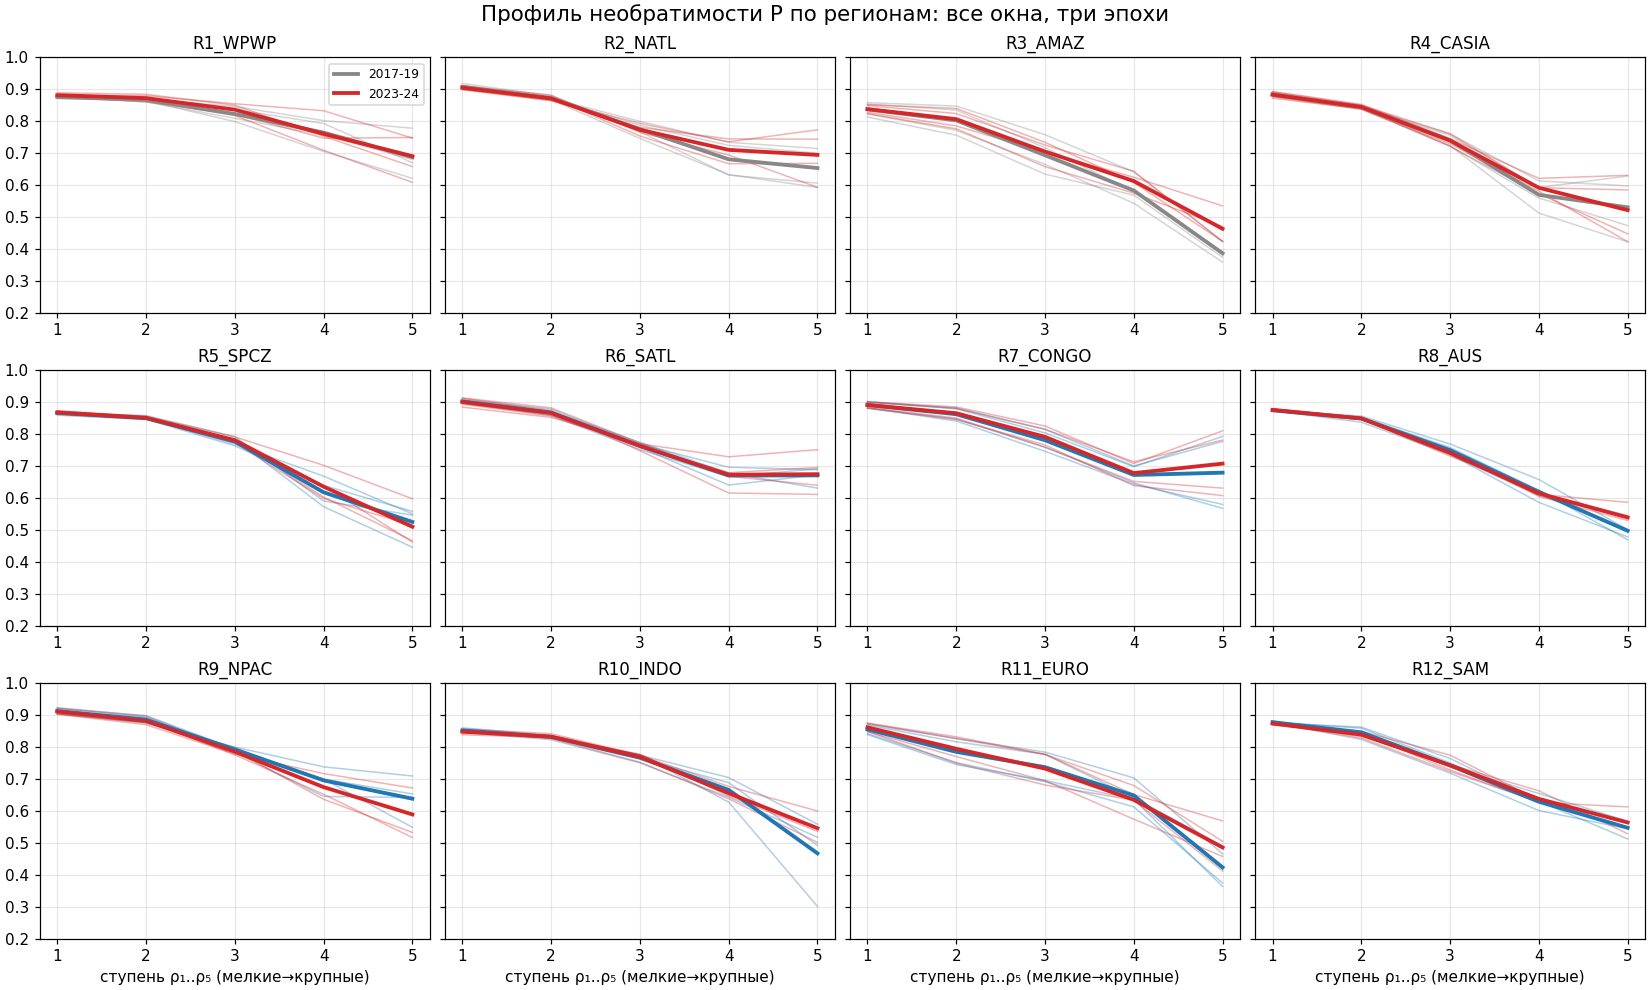
\includegraphics[width=\linewidth]{figures/fig_profiles_P.png}
\caption{Профили сопряжённости уровней $P$ для 12 регионов: тонкие линии --- отдельные сезонные окна, жирные --- средние по эпохам 2017--2019, 2021--2022 и 2023--2024~гг. Ступени 1--5 отвечают парам соседних октав от (50--100, 100--200~км) до (400--800, 800--1600~км).}
\label{fig:profiles}
\end{figure}

\subsection{Индекс асимметрии переноса: главный инвариант}
\label{sec:results:A}

Карта индекса $A$ (рис.~\ref{fig:map}) обнаруживает выраженный и физически осмысленный глобальный градиент: максимальные значения приурочены к влажно-конвективным океаническим режимам (Индийский океан 2{,}36; WPWP 2{,}26; SPCZ 2{,}19), промежуточные --- к штормтрекам (1{,}59--1{,}71) и конвективной суше (1{,}53--1{,}58), минимальные --- к аридным и умеренным внутриконтинентальным районам (Средняя Азия 1{,}41; Европа 1{,}38). Профили $A$ по уровням (рис.~\ref{fig:aprofiles}) воспроизводятся во всех трёх эпохах.

Статистический статус индекса --- самый прочный в программе. Региональная сигнатура подтверждена на выборке лет, не участвовавших в разработке дескриптора ($p=0{,}001$); индекс несёт информацию сверх спектра мощности \emph{и} сверх профиля сопряжённости $P$ (резидуализация, в обоих случаях $p=0{,}001$); результат не меняется при ограничении разрешёнными уровнями и при включении геометрических характеристик областей в резидуализацию ($p=0{,}001$). Попытка объяснить значения $A$ регрессией на средовые ковариаты (конвективный потенциал, доля суши, орография) даёт статистически значимую, но неустойчивую к исключению отдельных регионов модель; поэтому связь «максимум $A$ --- влажная конвекция над океаном» мы приводим как дескриптивную закономерность, а не как установленный закон.

\begin{figure}[t]
\centering
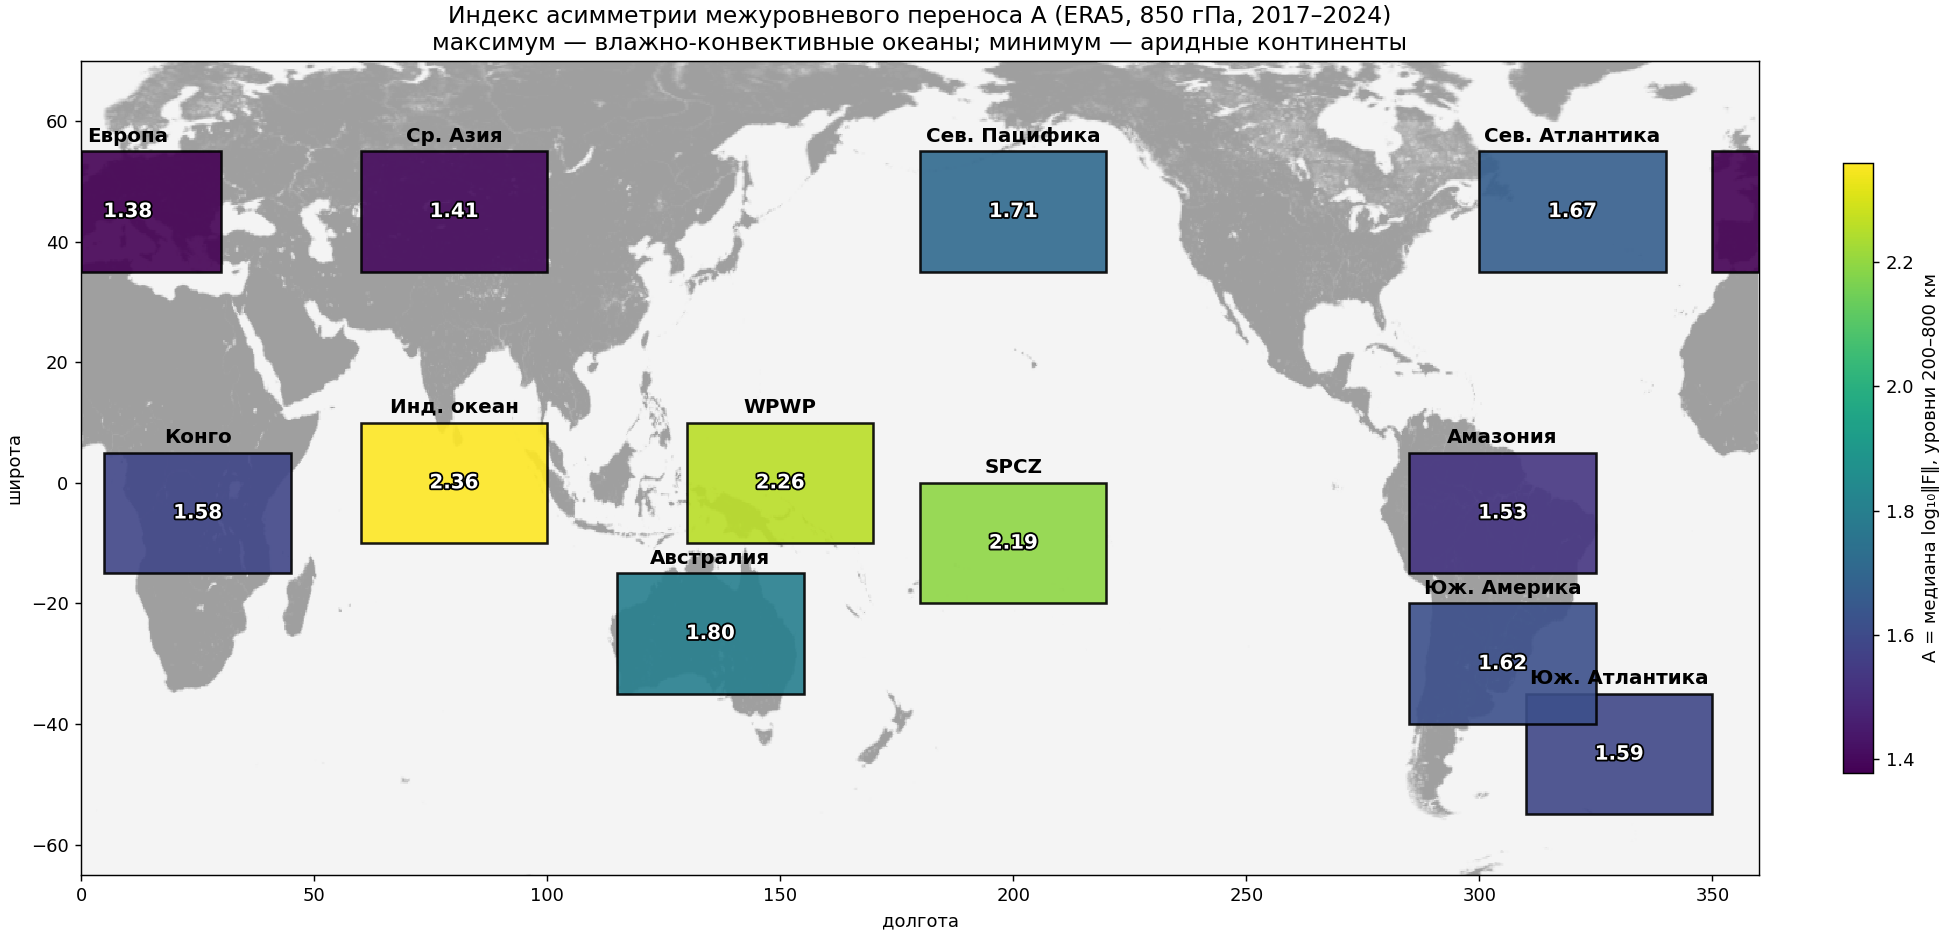
\includegraphics[width=\linewidth]{figures/figA_world_map.png}
\caption{Индекс асимметрии межуровневого переноса $A$ (медиана $\lg\lVert\cdot\rVert_F$ по разрешённым парам уровней 200--800~км; ERA5, 850~гПа, все окна 2017--2024~гг.). Числа --- значения $A$ для регионов.}
\label{fig:map}
\end{figure}

\begin{figure}[t]
\centering
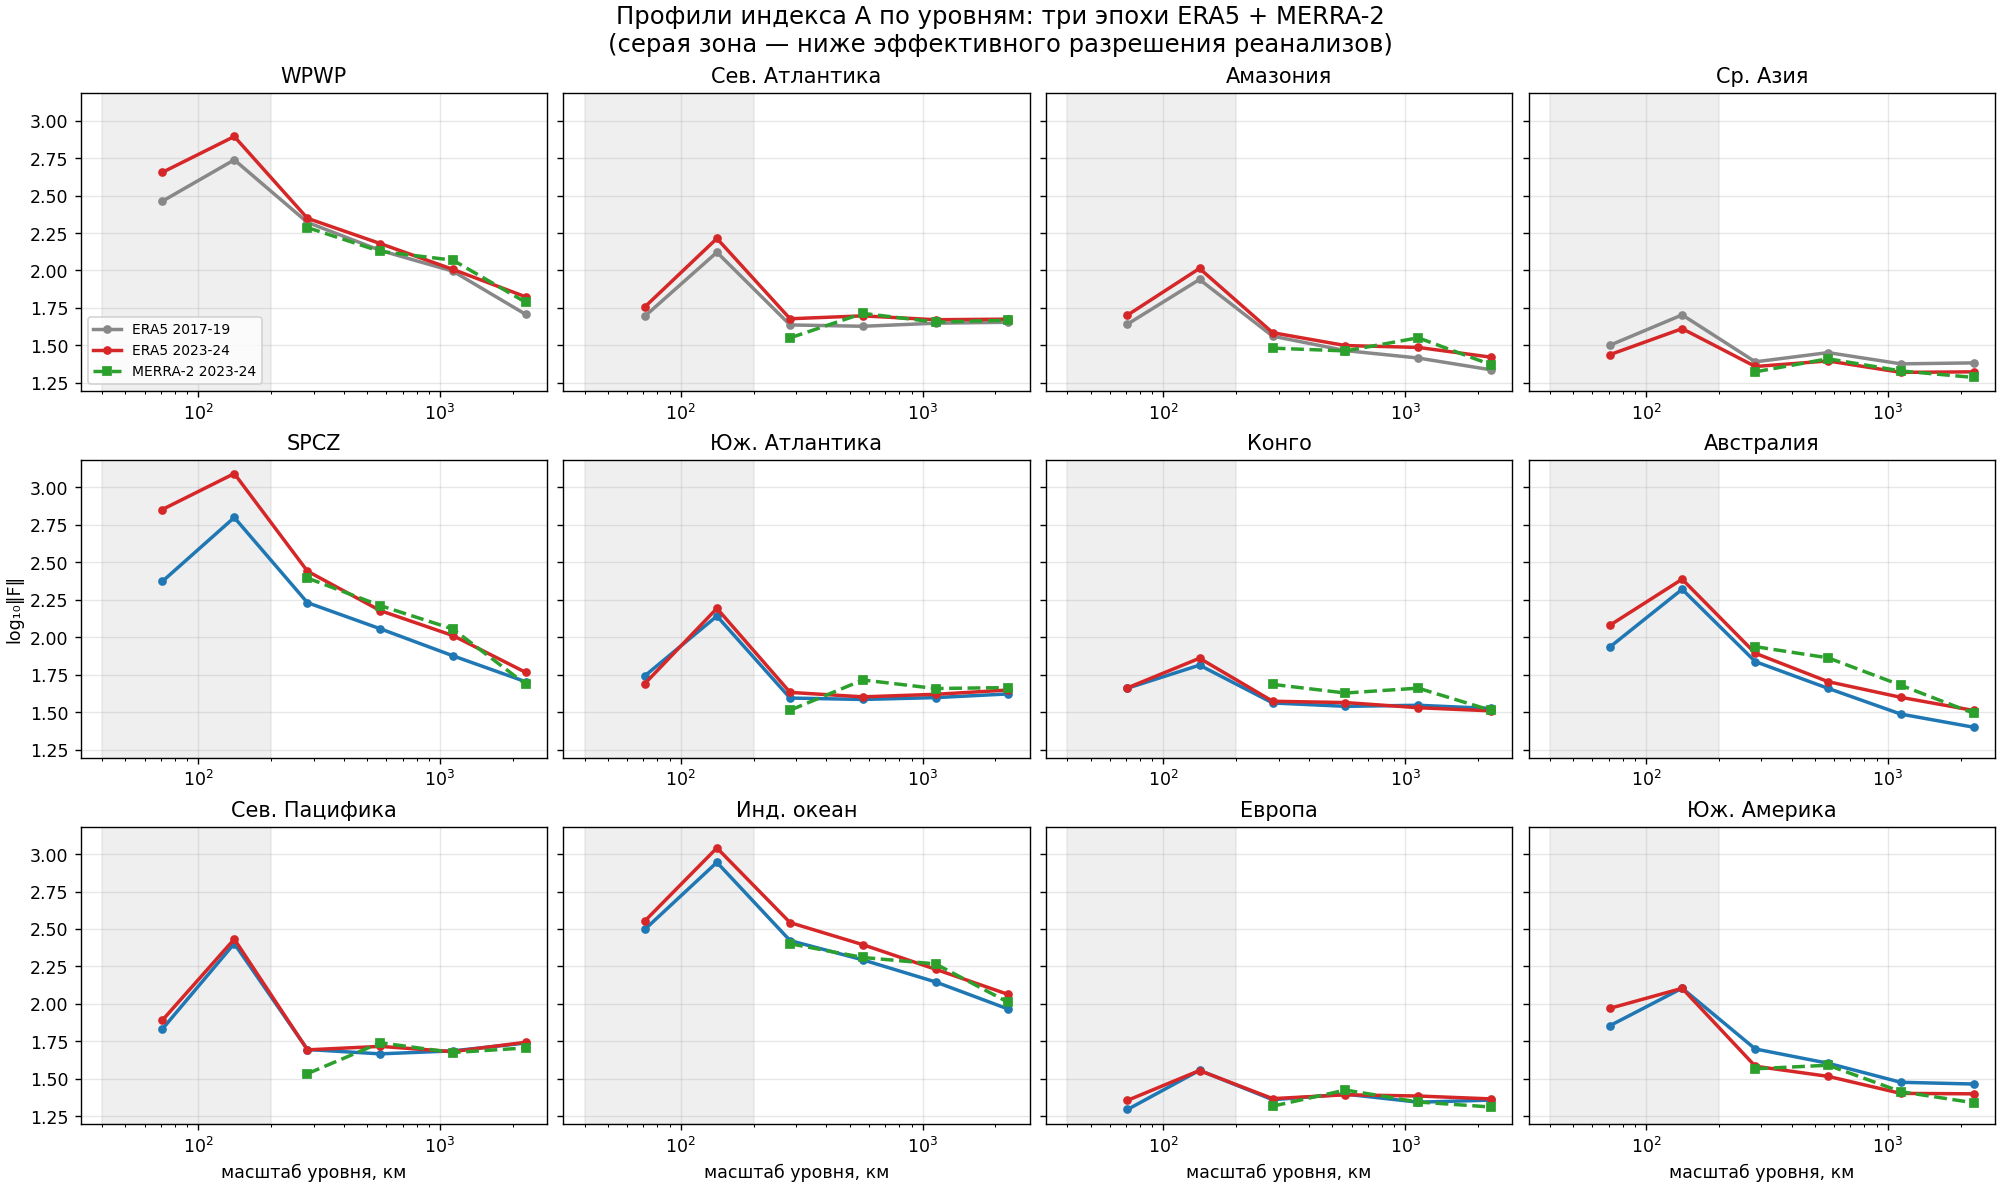
\includegraphics[width=\linewidth]{figures/figA_profiles.png}
\caption{Профили индекса $A$ по уровням: средние по эпохам ERA5 (2017--2019, 2021--2022, 2023--2024) и MERRA-2 (2023--2024, пунктир). Серая полоса --- масштабы ниже эффективного разрешения реанализов; сопоставление с MERRA-2 ведётся только по разрешённым уровням.}
\label{fig:aprofiles}
\end{figure}

\subsection{Межреанализная воспроизводимость}
\label{sec:results:merra}

Решающий контроль природы инварианта --- его воспроизводимость в реанализе с иной моделью и иной системой усвоения данных. Полный расчёт обоих дескрипторов по MERRA-2 (48 регион-окон 2023--2024~гг., разрешённые уровни) дал: региональная сигнатура $A$ в MERRA-2 значима ($p=0{,}001$; для $P$ также $p=0{,}001$), а региональная география индекса согласуется с ERA5 с ранговой корреляцией $\rho=0{,}93$ ($p<10^{-4}$; рис.~\ref{fig:merra}). Порядок регионов сохраняется практически полностью, включая тонкие различия внутри групп режимов. Тем самым инвариант не является артефактом конкретного реанализа; остающаяся общей для обоих продуктов наблюдательная сеть обсуждается в разд.~\ref{sec:discussion} как принципиальное ограничение любых реанализных климатологий.

\begin{figure}[t]
\centering
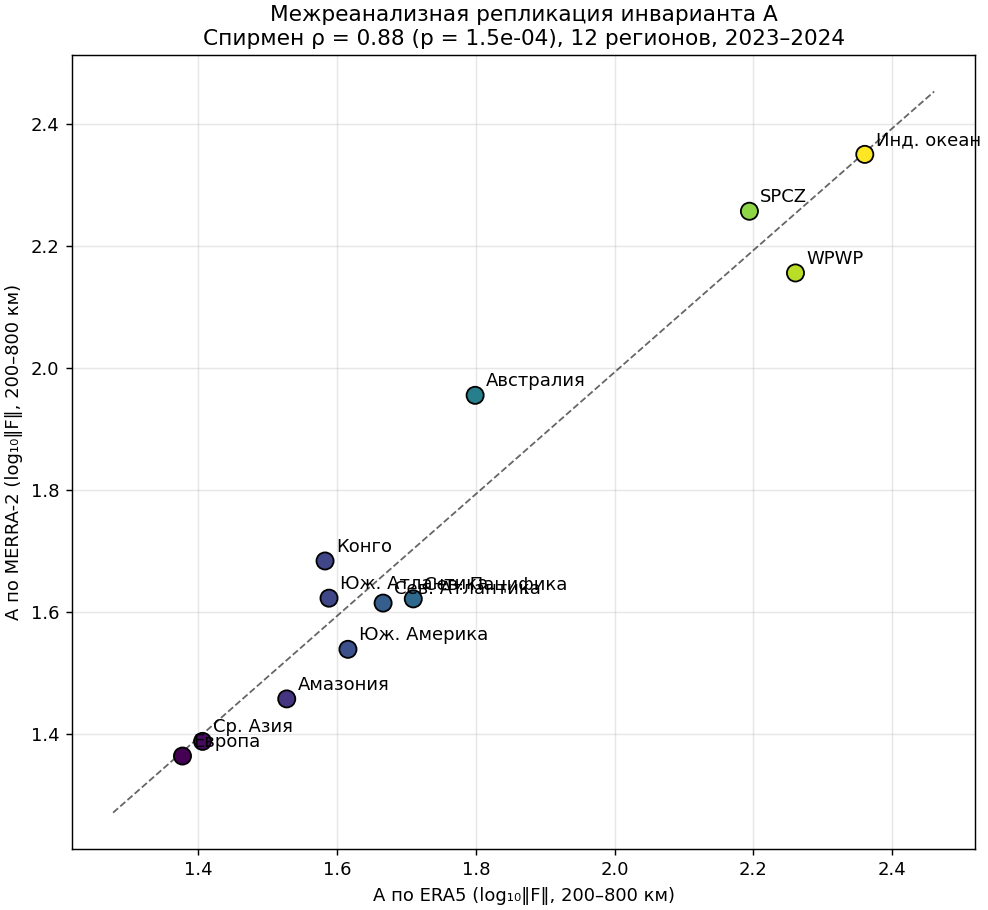
\includegraphics[width=0.62\linewidth]{figures/figA_cross_reanalysis.png}
\caption{Межреанализная воспроизводимость индекса $A$: значения по ERA5 (ось абсцисс) и MERRA-2 (ось ординат) для 12 регионов, 2023--2024~гг., разрешённые уровни 200--800~км.}
\label{fig:merra}
\end{figure}

\subsection{Региональный этюд: Конго и Амазония}
\label{sec:results:congo}

Наиболее показательный частный результат --- контраст двух главных очагов глубокой конвекции над сушей. При сходном режиме (экваториальная суша, высокая конвективная активность) и сходной плотности наблюдательной сети бассейн Конго демонстрирует высокую сопряжённость мезомасштаба с синоптическим уровнем ($\rho_5=0{,}71$), а Амазония --- аномально низкую ($\rho_5=0{,}46$); различие воспроизводится во всех эпохах и в MERRA-2. На октавных картах (рис.~\ref{fig:octaves}) видно то же качественно: во внетропическом циклоне фронтальная полоса прослеживается согласованно на всех уровнях, тогда как в амазонском режиме крупномасштабные карты активности почти не предсказывают размещения мезомасштабной изменчивости. Двум очагам конвекции соответствуют, таким образом, \emph{разные архитектуры} межуровневой организации --- различие, невидимое ни для спектров, ни для стандартных конвективных индексов, но устойчиво фиксируемое предлагаемыми дескрипторами. Механизм этого контраста (роль восточных волн, сдвига ветра, суточного хода, орографического обрамления бассейнов) --- открытый вопрос для регионального анализа.

\begin{figure}[t]
\centering
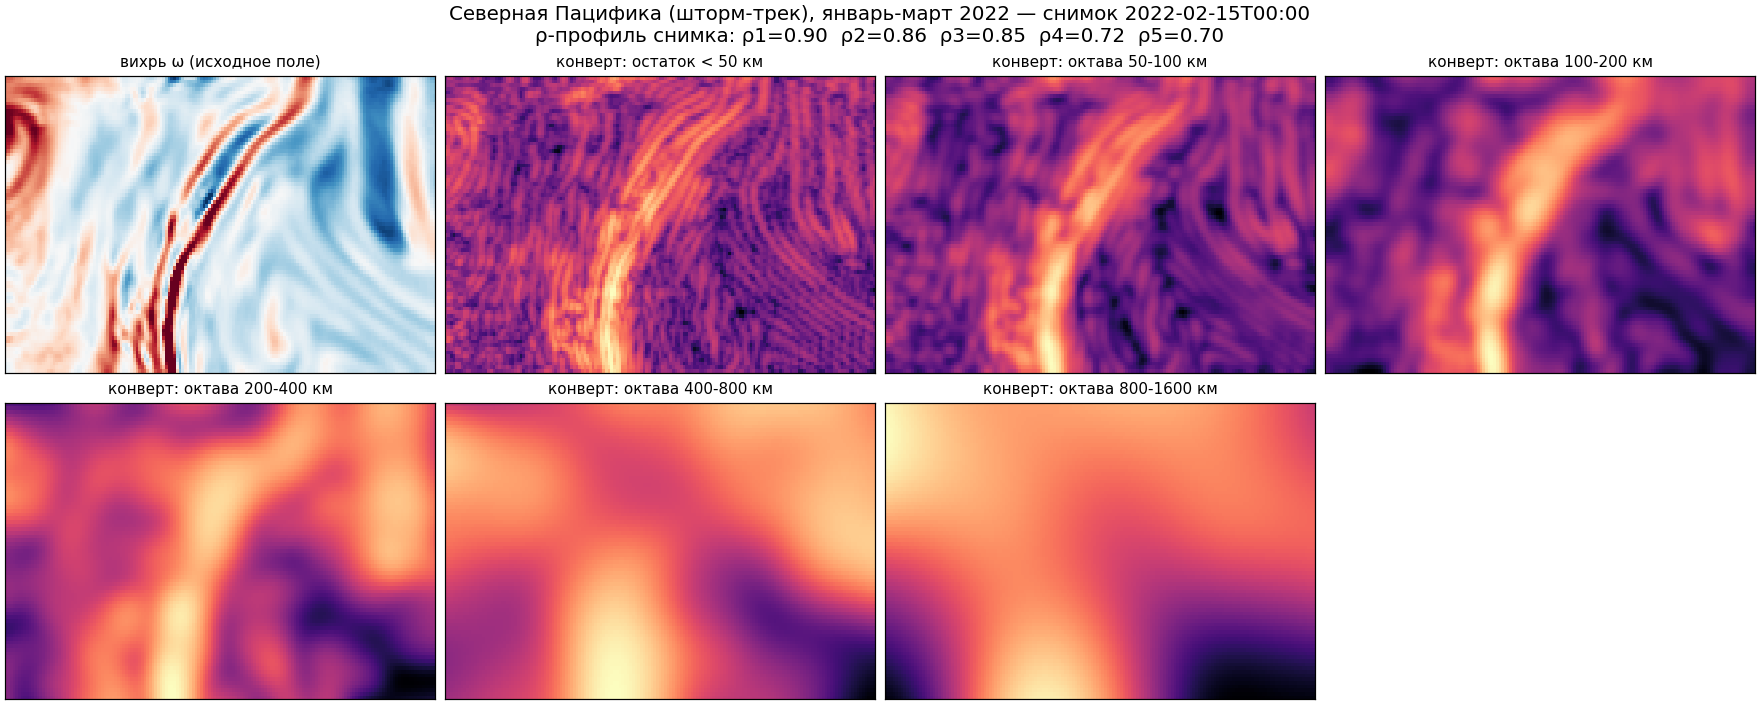
\includegraphics[width=\linewidth]{figures/octave_maps_R9_NPAC_W7_2022JFM.png}\\[2pt]
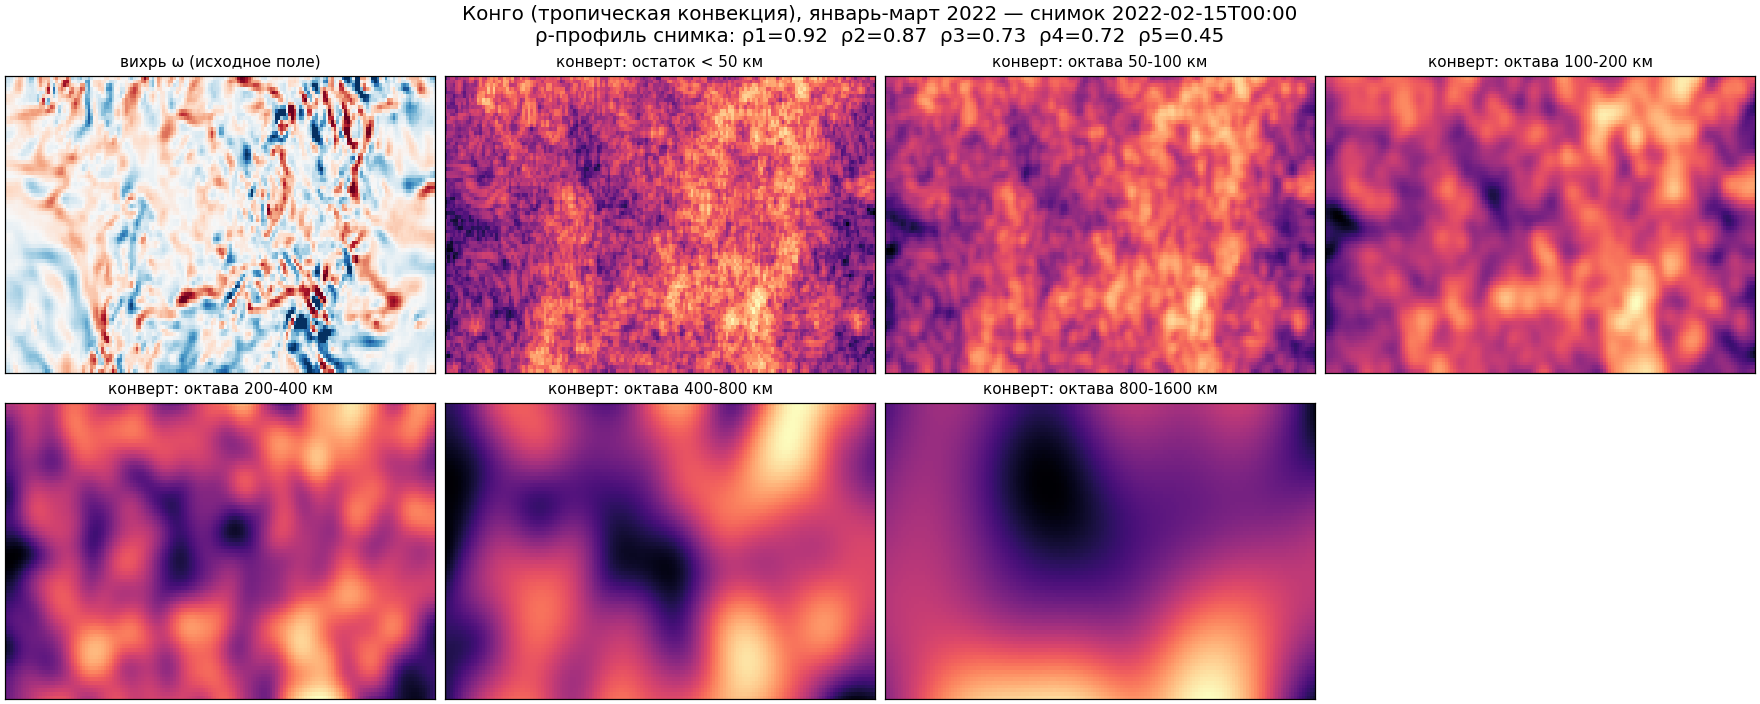
\includegraphics[width=\linewidth]{figures/octave_maps_R7_CONGO_W7_2022JFM.png}
\caption{Карты активности октавных уровней для одного срока (15.02.2022): вверху --- северотихоокеанский штормтрек (фронтальная структура согласованно «светится» на всех уровнях, высокая сопряжённость), внизу --- бассейн Конго (мезомасштабная активность слабее подчинена крупным уровням). Цветовая шкала каждой панели своя (логарифм огибающей); сопряжённость измеряет совпадение географии, а не амплитуды.}
\label{fig:octaves}
\end{figure}

\begin{table}[t]
\centering
\caption{Сводка подтверждающих проверок инвариантов (перестановочные тесты кластеризации, 999 перестановок; «независимые годы» --- выборки, не участвовавшие в постановке соответствующего дескриптора).}
\label{tab:tests}
\small
\begin{tabular}{@{}p{0.42\linewidth}p{0.23\linewidth}p{0.25\linewidth}@{}}
\toprule
Проверка & Профиль $P$ & Индекс $A$\\
\midrule
Региональная сигнатура, независимые годы & $p=0{,}001$ & $p=0{,}001$\\
Сверх спектра мощности & $p=0{,}029$; после контроля геометрии $p=0{,}10$ & $p=0{,}001$ (устойчив)\\
Сверх семифрактальных уровней \cite{Krenke2019} & $p=0{,}001$ & ---\\
Сверх скаттеринг-статистик & $p=0{,}026$ & ---\\
Сверх профиля $P$ & --- & $p=0{,}001$\\
Только разрешённые уровни ($\geq$200 км) & $p=0{,}002$ & $p=0{,}001$\\
Сигнатура в MERRA-2 & $p=0{,}001$ & $p=0{,}001$\\
Согласие географии ERA5/MERRA-2 & --- & $\rho=0{,}93$, $p<10^{-4}$\\
\bottomrule
\end{tabular}
\end{table}

\section{Отрицательные результаты и границы применимости}
\label{sec:negative}

Программа проверок дала обширный каталог отрицательных результатов, которые мы считаем равноправной частью итога (табл.~\ref{tab:negative}). Кратко прокомментируем главные. (а)~Связь дескрипторов с истинным межмасштабным потоком кинетической энергии (вычисленным методом огрубления \cite{Germano1992,Aluie2018} с независимой проверкой кода на численном эксперименте) отвергнута: стандартные суррогаты потока многократно информативнее. (б)~Универсальной зависимости формы профилей от средовых ковариат нет: перенормировки масштабной оси, очистка от зональной полосчатости и переход к полю влагопереноса не «упрощают» профили до единой кривой --- напротив, переход к влагопереносу усиливает региональные различия. (в)~Мгновенной локальной связи индекса $A$ с осадками нет; режимная антикорреляция на пятисуточном сглаживании по срокам согласуется с известным циклом накопления--сброса конвективной энергии ($\sim$1--2~сут восстановления \cite{Masunaga2012}), однако попытка идентифицировать динамическое уравнение «источник--сток» не прошла проверку на независимых регионах, а масштаб времени релаксации частично воспроизводится и инерцией самого оценивателя; вопрос остаётся открытым. (г)~Вертикального переноса инварианта нет: на 500~гПа региональная география $A$ иная --- дескрипторы уровнеспецифичны. (д)~Информации о невязке влагобюджета реанализа дескрипторы не несут: невязка ERA5 определяется инкрементами усвоения \cite{Trenberth1991,Mayer2021}, и никакие межуровневые характеристики циркуляции её не предсказывают.

\begin{table}[t]
\centering
\caption{Каталог отрицательных результатов программы и исправлений предшествующей публикации.}
\label{tab:negative}
\small
\begin{tabular}{@{}p{0.58\linewidth}p{0.36\linewidth}@{}}
\toprule
Гипотеза & Итог проверки\\
\midrule
Дескрипторы отслеживают истинный поток энергии между масштабами & отвергнута (суррогаты потока в $\sim$50 раз информативнее)\\
Центральное утверждение \cite{Sotiriadi2026} (замыкание $\Lambda_b\sim\Pi_b$) & \textbf{ретрагировано}: прокси не являлся потоком; статистика завышена биннингом и подгонкой знака; единственное проходящее окно из шести\\
Скалярная свёртка со знаком (величина $\Lambda$ из \cite{Sotiriadi2026}) & не несёт региональной информации ($p=0{,}7$)\\
«Интегрируемость» связи уровней (согласованность путей время$\times$масштаб) & ретрагирована после корректного суррогатного нуля, сохраняющего временной спектр\\
Универсальный закон формы профилей от ковариат (CAPE, суша, орография) & отвергнута (форма не коллапсирует)\\
Мгновенный локальный источник $A$ в осадках & отвергнута ($0/32$ окон)\\
Динамическое уравнение «накопление--сброс» для $A$ & не установлено (нет предсказательной силы на независимых регионах)\\
Вертикальная инвариантность (перенос на 500~гПа) & отвергнута (уровнеспецифичность)\\
Вклад дескрипторов в замыкание влагобюджета & отвергнута (медианный прирост $-0{,}018$, $p=0{,}92$)\\
Упрощение профилей при переходе к влагопереносу & обратный эффект (различия усиливаются)\\
\bottomrule
\end{tabular}
\end{table}

\section{Обсуждение}
\label{sec:discussion}

\subsection{Исправления предшествующей публикации}
\label{sec:corrections}

Центральное эмпирическое утверждение работы \cite{Sotiriadi2026} --- «замыкание» $\Lambda_b\sim\Pi_b$ в инерционном интервале ERA5 --- не выдержало проверки против истинного потока энергии и ретрагируется (табл.~\ref{tab:negative}, строки 2--4): использованный там спектральный прокси не являлся потоком, статистическая обработка (биннинг, внутривыборочное выравнивание знака) завышала связь, а положительный результат был получен в единственном из шести временных окон. Терминология «профиль необратимости» и «кривизна» также признана неудачной: первая статистика симметрична и переименована в профиль сопряжённости, вторая является эмпирическим индексом асимметрии переноса без претензий на геометрическую онтологию. Методологический урок мы считаем частью результата: сочетание заранее фиксируемых протоколов, подтверждения на независимых данных и внешнего методического аудита позволило за конечное число шагов отделить устойчивое ядро от артефактов --- включая ретракцию одного «красивого» промежуточного результата (об «интегрируемости»), причиной которого оказался некорректно построенный суррогатный нуль.

\subsection{Географический смысл инвариантов}

Предложенные дескрипторы измеряют то, что можно назвать \emph{архитектурой иерархии} регионального циркуляционного режима. Профиль $P$ отвечает на вопрос, насколько размещение мезомасштабной изменчивости подчинено крупным уровням; индекс $A$ --- насколько необратим переход между уровнями описания. Второй имеет прямую интерпретацию в терминах классической географической проблемы генерализации: $A$ есть мера того, сколько пространственной информации о мезоструктуре территории принципиально теряется при обобщении и не восстанавливается статистической детализацией. Высокие значения $A$ над влажно-конвективными океанами означают, что мезомасштабная организация там формируется «снизу», процессами, слабо детерминированными крупномасштабным полем; низкие значения над аридными континентами --- что иерархия уровней близка к статистически обратимой. Для практики отсюда следуют две области приложения: объективное районирование по межуровневой организации (дескрипторы дают компактный, воспроизводимый признак режима, различающий даже территории со сходными спектрами --- ср. Конго и Амазонию) и оценка априорной пригодности статистической детализации (даунскейлинга): регионы с высоким $A$ --- территории, где восстановление мезоструктуры по крупномасштабным полям наименее обосновано.

В терминах программы Пузаченко полученные характеристики удовлетворяют операциональному определению инварианта динамики геосистем \cite{Puzachenko2010}: они устойчивы во времени (сезоны, годы, фазы ЭНСО), различают территории и не сводятся к ранее известным характеристикам организации --- спектрам, фрактальным размерностям и спектральным уровням \cite{Krenke2019}. Настоящую работу мы рассматриваем как шаг той же исследовательской линии: от выделения уровней --- к измерению их взаимодействия.

\subsection{Гипотеза о связи с предсказуемостью}

Литература о росте ошибок прогноза отводит межмасштабному взаимодействию роль канала, по которому неопределённость мелких масштабов заражает синоптический уровень \cite{Lorenz1969,Zhang2007,RotunnoSnyder2008,Judt2020}. Региональная климатология этого взаимодействия, построенная здесь по данным реанализов, естественно порождает проверяемую гипотезу: региональные различия сопряжённости и асимметрии уровней должны коррелировать с региональными различиями скорости роста ошибок в ансамблевых системах прогноза. Мы намеренно оставляем это утверждение в статусе гипотезы: её проверка требует сопоставления с ансамблевыми данными и составляет самостоятельную задачу.

\subsection{Ограничения}

Главное принципиальное ограничение --- общая для всех реанализов зависимость от наблюдательной сети: воспроизводимость инварианта в двух независимых системах усвоения (ERA5, MERRA-2) исключает артефакт конкретной модели, но не артефакт географии наблюдений как таковой \cite{BonavitaLaloyaux2020}. Полное снятие этого ограничения требует расчёта дескрипторов по свободным (безусвоенческим) модельным экспериментам. Далее: анализ ограничен уровнем 850~гПа (уровнеспецифичность показана прямо), двумя сезонами, фиксированной сеткой регионов; мелкие октавы лежат ниже эффективного разрешения реанализов и исключены из выводов; наконец, дескрипторы остаются статистическими характеристиками --- динамическая модель, порождающая их региональные различия, не построена.

\section{Выводы}
\label{sec:conclusion}

1.~Предложены два компактных дескриптора межуровневой организации атмосферной циркуляции: профиль сопряжённости октавных уровней $P$ и индекс асимметрии межуровневого переноса $A$; второй, по-видимому, не имеет прямых аналогов в литературе.

2.~Оба дескриптора образуют устойчивые региональные сигнатуры (сезоны, годы, фазы ЭНСО; $p=0{,}001$ на независимых выборках); индекс $A$ несёт информацию сверх спектра мощности, сверх профиля $P$ и сверх спектральных уровней в смысле \cite{Krenke2019}, и устойчив ко всем применённым контролям.

3.~Региональная география индекса $A$ воспроизводится в независимом реанализе MERRA-2 ($\rho=0{,}93$): инвариант характеризует атмосферу, а не систему усвоения данных. Максимум асимметрии --- влажно-конвективные океаны, минимум --- аридные континенты; Конго и Амазония демонстрируют качественно разные архитектуры иерархии при сходных режимах.

4.~Каталог отрицательных результатов очерчивает границы: дескрипторы не измеряют поток энергии, не подчиняются простому ковариатному закону, уровнеспецифичны и не несут информации о невязке влагобюджета; центральное утверждение предшествующей публикации автора ретрагировано.

5.~Полученные характеристики удовлетворяют операциональному определению инварианта динамики геосистем и продолжают линию школы Пузаченко --- от выделения иерархических уровней к измерению их взаимодействия; ближайшие приложения --- объективное районирование, априорная оценка пригодности даунскейлинга и проверяемая гипотеза о связи с региональными пределами предсказуемости.

\paragraph{Данные и код.} Все протоколы (включая журнал отклонений и материалы независимого аудита), код экспериментов, таблица полной исследовательской программы (73 эксперимента) и численные результаты открыты в репозитории программы (ветка gen3): \url{https://github.com/Theclimateguy/Shroedinger}.

\printbibliography[title={Список литературы}]

\end{document}
